\documentclass[12pt]{amsart}
\usepackage{geometry}                % See geometry.pdf to learn the layout options. There are lots.
\geometry{letterpaper}                   % ... or a4paper or a5paper or ... 
%\geometry{landscape}                % Activate for for rotated page geometry
%\usepackage[parfill]{parskip}    % Activate to begin paragraphs with an empty line rather than an indent
\usepackage{graphicx}
\usepackage{amssymb}
\usepackage{epstopdf}
\usepackage{fullpage}
\usepackage{amsmath}
\usepackage{mathtools}
%\usepackage{parsetree}
\usepackage{qtree}
\DeclareGraphicsRule{.tif}{png}{.png}{`convert #1 `dirname #1`/`basename #1 .tif`.png}
\usepackage{fancyhdr}
\setlength{\headheight}{15pt}
\setlength{\headsep}{25pt}
\setlength{\footskip}{35pt}
\pagestyle{fancy}

\renewcommand{\rmdefault}{ptm}

\title{cs482 Project Proposal}

\pagestyle{fancy}

\begin{document}
\begin{titlepage}
\begin{center}

\textsc{\LARGE cs482\\Computer Vision }\\[1.5cm]

% Title
%\HRule \\[0.4cm]

{ 
\Large {\bfseries Project Report}
\small




Kevin St.Andrie

{\footnotesize (kstandri@masonlive.gmu.edu)}

Travis Hile

Martin Taheri

Jeremiah Howdeshell

Chris Sahno }\\[1.5cm]

%\HRule \\[1.5cm]

% Author and supervisor

\vfill

% Bottom of the page
{\large \today}

\end{center}

\end{titlepage}
\fancyfoot{}
\newpage
\setcounter{page}{1}
\fancyhf{}
\fancyhead{} % clear all header fields 
\fancyhead[CO,CE]{} 
\fancyhead[RO,LE]{Project Report}
\fancyhead[LO,RE]{\thepage}
\renewcommand{\headrulewidth}{0.0pt} 
\renewcommand{\footrulewidth}{0.0pt}

\newpage
\thispagestyle{empty}
\mbox{}
\pagebreak

\section{Objective}
Our stated objective was to investigate and understand the methods used to develop panoramic and composite images and to adapt these techniques into a portable code library which could conceivably be run on a smartphone (such as an Android device).

\section{Methodology}
\subsection{Dataset Acquisition}
The first step was to acquire our dataset. Using a relatively new 10 megapixel digital camera and a tripod, we captured 96 images. By using the same camera and focusing on one object for each set, we maximized the number of matching features from which to build a composite image.
\begin{itemize}
	\item 40 images were taken at $10^{\circ}$ increments from the same fixed position using the tripod along the path between the Research building and the Arts building.
	\item 27 images were taken the Engineering building from different vantage points, in order to generate parallax errors issues.
	\item 16 images were taken of the Research building from many different vantage points, in order to generate parallax errors issues.
	\item 13 images were taken of one the many sidewalks on campus, for parallax issues and to acquire human ghosts.
\end{itemize}

\begin{figure}[htbp]
\begin{center}
\includegraphics[scale =.5]{rptImages/100_2992.jpg}\includegraphics[scale =.5]{rptImages/100_2993.jpg}\includegraphics[scale =.5]{rptImages/100_2994.jpg}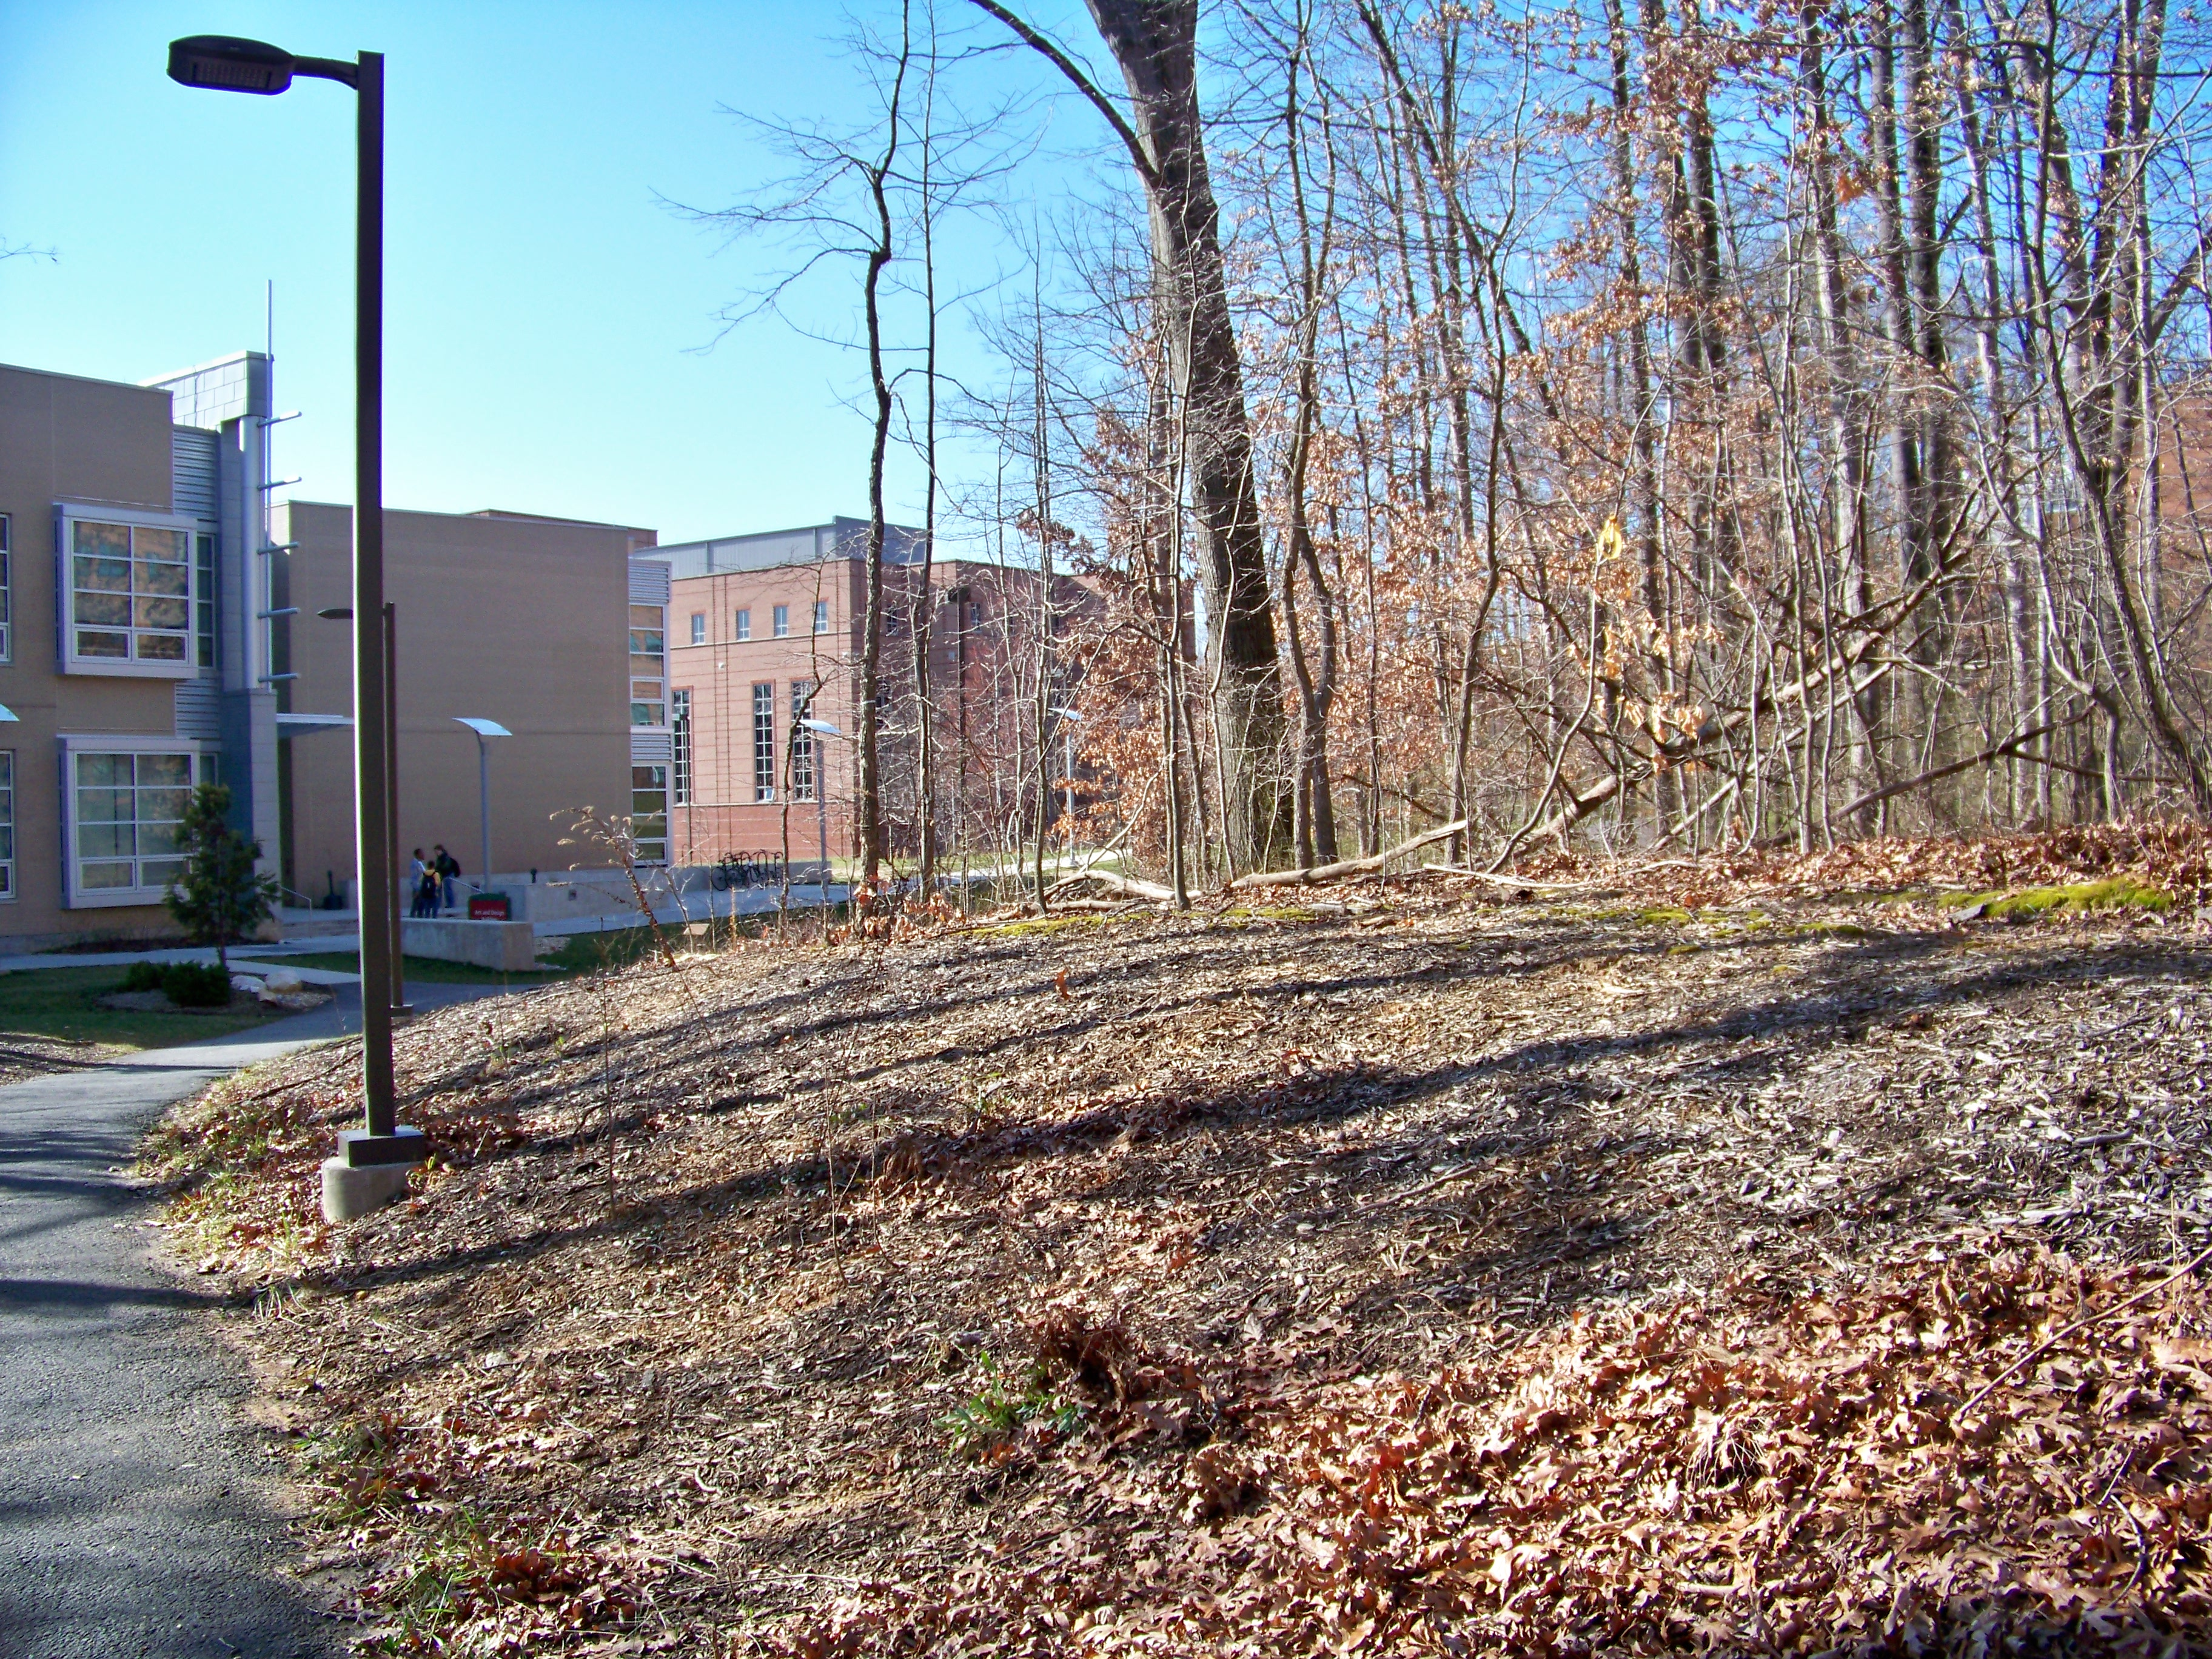
\includegraphics[scale =.5]{rptImages/100_2995.jpg}
\caption{A series of images from the control dataset. $10^{\circ},20^{\circ},30^{\circ},40^{\circ}$ from the origin frame, respectively.}
\label{default}
\end{center}
\end{figure}

\begin{figure}[htbp]
\begin{center}
\includegraphics[scale =.5]{rptImages/100_3066.jpg}\includegraphics[scale =.5]{rptImages/100_3067.jpg}\includegraphics[scale =.5]{rptImages/100_3068.jpg}\includegraphics[scale =.5]{rptImages/100_3069.jpg}
\caption{A series of images from the control dataset. Note the humans in the scenes, and the difference in camera angles.}
\label{default}
\end{center}
\end{figure}

\subsection{Design}
Our initial research showed that the effort required to develop a library of our own design was beyond the time and scope of the course. Simply implementing some of the algorithms by ourselves (such as RANSAC) would have been a large undertaking.

We settled on focusing on our primary objective, which was to investigate and understand the methods for stitching images. To this end, we used two computer vision libraries, Boofcv and OpenCV.

We built two programs, one for Android end users using the Boofcv library, and a proof of concept using the OpenCV library. Output images used in this report will be from the Python-OpenCV set.

\section{How do I do that?}



\end{document}
